\begin{pastexam}[label={px:ntu-114-bmei-ca-03}]{臺大生醫電資所 114 學年度 第 3 題}
（問答）

(6\%) Please draw the binary search tree after successively inserting keys 3, 9, 8, 6, 5, 4, 1, 2, 7 into an initially empty tree.
\end{pastexam}

\begin{pastsoln}
每個鍵從根往下走，比節點小往左、大往右，走到空位就放（資結書第~9.2~節）：
\begin{itemize}
\item $3$：根。
\item $9$：$> 3$，放 $3$ 的右。
\item $8$：$> 3$、$< 9$，放 $9$ 的左。
\item $6$：$> 3$、$< 9$、$< 8$，放 $8$ 的左。
\item $5$：$> 3$、$< 9$、$< 8$、$< 6$，放 $6$ 的左。
\item $4$：$> 3$、$< 9$、$< 8$、$< 6$、$< 5$，放 $5$ 的左。
\item $1$：$< 3$，放 $3$ 的左。
\item $2$：$< 3$、$> 1$，放 $1$ 的右。
\item $7$：$> 3$、$< 9$、$< 8$、$> 6$，放 $6$ 的右。
\end{itemize}
\begin{center}
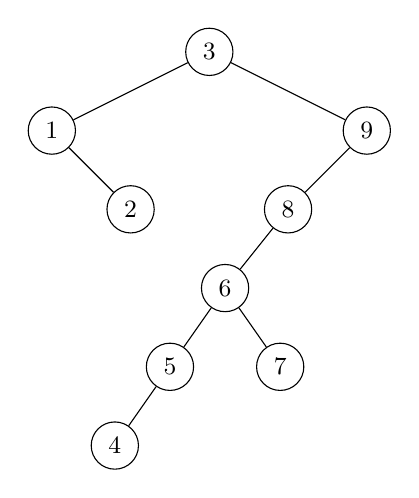
\begin{tikzpicture}[every node/.style={circle,draw,inner sep=1pt,minimum size=6mm,font=\small},level distance=10mm,edge from parent/.style={draw},level 1/.style={sibling distance=40mm},level 2/.style={sibling distance=20mm},level 3/.style={sibling distance=16mm},level 4/.style={sibling distance=14mm}]
\node {3}
  child {node {1} child[missing] child {node {2}}}
  child {node {9}
    child {node {8}
      child {node {6}
        child {node {5} child {node {4}} child[missing]}
        child {node {7}}}
      child[missing]}
    child[missing]};
\end{tikzpicture}
\end{center}
檢查：中序走訪得 $1, 2, 3, 4, 5, 6, 7, 8, 9$，由小到大，是合法的二元搜尋樹。 右邊 $9 \to 8 \to 6 \to 5 \to 4$
一路往左，因為這幾個鍵是遞減插入的。
\end{pastsoln}
